\section{Introduction}
\label{sec:Introduction}

Safety and mission-critical DRE systems are used in a variety of domains such as avionics, locomotive control, industrial and medical automation. Given the increasing role of software in such systems, growing both in size and complexity, utilizing predictable and dependable software is critical for system safety. To mitigate this complexity, model-driven, component-based software development has become an accepted practice. Applications are built by assembling together small, tested component building blocks that implement a set of services. Models describe what these component blocks are, what interfaces they have, how they are built, how they interact and how they are deployed to realize the domain-specific application. 

Complex, managed systems, e.g. a fractionated spacecraft following a mission timeline and hosting distributed software applications expose heterogeneous concerns such as strict timing requirements, complexity in deployment, repair and integration; and resilience to faults. High-security and time-critical software applications hosted on such platforms run concurrently with all of the system-level mission management and failure recovery tasks that are periodically undertaken on the distributed nodes. Once deployed, it is often difficult to obtain low-level access to such remote systems for run-time debugging and evaluation. These types of systems therefore demand advanced design-time modeling and analysis methods to detect possible anomalies in system behavior, such as unacceptable response time, before deployment. 

Our team has designed and prototyped a full information architecture called \textbf{D}istributed \textbf{RE}al-time \textbf{M}anaged \textbf{S}ystem (DREMS) \cite{ISIS_F6_Aerospace:12,DREMS13Software} that addresses requirements for rapid component-based application development. In prior work, we have described the design-time modeling capability \cite{ISIS_F6_SFFMT:13}, and the component model used to build and execute applications \cite{ISIS_F6_ISORC:13}.
%This architecture consists of a design-time tool suite for modeling, analysis, synthesis, integration, debugging, testing, and maintenance of application software built from reusable components. The architecture also provides a run-time software platform for deploying, managing, and executing application software on a network of mobile computing nodes. 
The formal modeling and analysis method presented in this paper focuses on applications that rely on this foundational architecture. The principle behind design-time analysis here is to map the structural and behavioral specifications of the system under analysis into a formal domain for which analysis tools exist. The key is to use an appropriate model-based abstraction such that the mapping from one domain to another remains valid under successive refinements in system development such as code generation. 
%This abstraction includes formalizing (1) the structure of component building blocks, (2) the semantics of component interaction patterns, and (3) the abstract temporal behavior of application components. 
The analysis must ensure that as long as the assumptions made about the system hold, the behavior of the system lies within the safe regions of operation.  The results of this analysis will enable system refinement and re-design if required, before actual code development. 

%\AD{Suggested Problem Statement: The principle behind design time analysis is to map the model of the system under analysis into a formal domain for which analysis tools exist. Key here is to use appropriate model based abstraction such that the mapping from one domain to other domain remains valid under successive refinements such as code-generation. For our work, we have chose the colored petri net as the formal domain - please describe why. }

%\AD{Please describe three different points from the abstract here and show how they lead to verification driven workflow. Make sure to identify the contributions of this paper.}

\vspace{-0.12in}
\begin{figure}[ht]
\centering
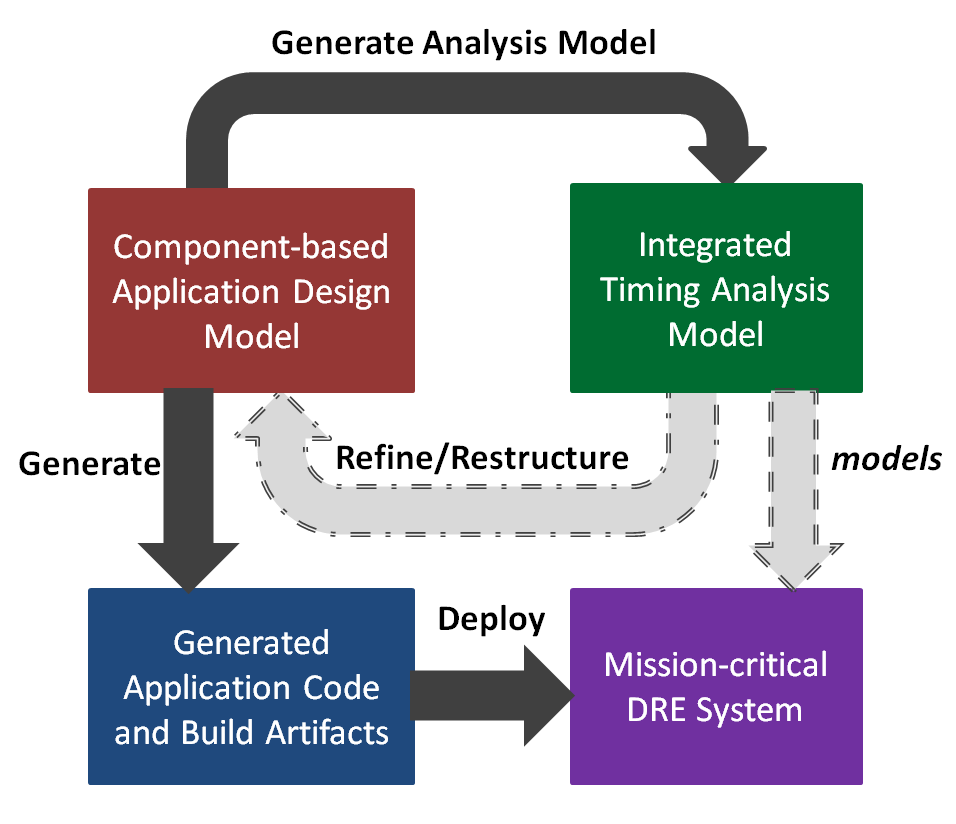
\includegraphics[width=0.38\textwidth]{big_picture}
\caption{Verification-driven Workflow}
\label{fig:big_picture}
\vspace{-0.16in}
\end{figure}

Figure \ref{fig:big_picture} shows a Verification-driven workflow for component-based software development. Application developers use domain-specific modeling languages to model the component assembly, interaction patterns, component execution code, sequence of operations, and associated temporal properties such as estimated execution times, deadlines etc. Using such application-specific parameters in the \textit{design} model, a Colored Petri net-based (CPN) \cite{CPN} \textit{analysis} model is generated. The system behavior is analyzed to check properties like lack of deadlocks, deadline violations etc. %The results of this analysis help improve the structure of the application, enabling safe deployment of dependable components that are known to operate within system specifications.  

The remainder of this paper is organized as follows. Section~\ref{sec:Related_Research} presents existing research relating to this paper and explains how this approach is different; Section \ref{sec:Background} provides a brief background on the DREMS Infrastructure and on the CPN formalism; Section \ref{sec:Problem_Statement} discusses the problem statement that is evaluated; Section \ref{sec:CPN_Modeling} elaborates on how this architecture is abstracted and modeled using CPN; Section \ref{sec:State_Space_Analysis} investigates the utility and scalability of this approach in detecting deadline violations, calculating worst-case trigger-response times and determining partial thread execution orders; Section \ref{sec:Model_Generation} briefly describes how the analysis model can be generated; Sections \ref{sec:Discussion}, \ref{sec:Future_Work} and \ref{sec:Conclusions} present a brief discussion of the presented results, future extensions to the proposed approach and concluding remarks respectively.